\documentclass[catalog.tex]{subfiles}

% do not write anything in the preamble

\begin{document}

\def\pbname{YOLO} %change this, do not use any number, just the name

\section{\pbname} 

% only for overview, so short description (no more than 1-2 lines)
\begin{overview}
\item [Algorithm:] YOLO
	% -	must match the label of the algorithm 
	% - when writing more than one algo use alg:\currfilebase_a, alg:\currfilebase_b, etc.
\item [Input:] A training set, A full image
\item [Complexity:] N/A
\item [Data structure compatibility:] N/A
\item [Common applications:] Object detection
\end{overview}


\begin{problem}{\pbname}
	YOLO (You Only Look Once) is an unified, real-time object detection algorithm that does all predictions directly from full images, the bounding boxes, as well as related class probabilities in a single evaluating process. 
\end{problem}
\subsection*{Description}
\subsubsection*{Introduction}
\par YOLO regards object detection as a single regrssion problem, where input is image pixels, output is bounding box coordinates and class probabilities. YOLO is trained jointly based on the loss function which corresponds to the performance of detection. The overall process of YOLO algorithm can be simplified as
\begin{figure}[h]
	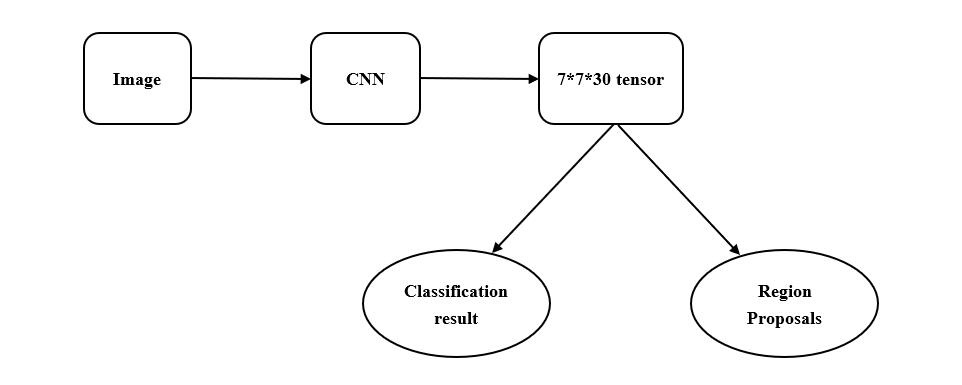
\includegraphics[width=\textwidth]{problem-117_a.jpg}
	\caption{Simplification of YOLO}
\end{figure} 
\newpage
\subsubsection*{Unified Detection}
\par YOLO sees the image as an $S \times S$ grid. If the center of an object in the image falls into a cell, the detection will be processed on such cell. Every cell evaluates $B$ bounding boxes and respective confidence scores. The confidence score is defined as $\operatorname{Pr}(\text { Object }) \cdot \mathrm{IOU}_{\text {pred }}^{\text {truth }}$. If the bounding box contains object,$\operatorname{Pr}(\text { Object })=1$, else $\operatorname{Pr}(\text { Object })=0$
\par There are 5 values for a bounding box, $x,y,w,h$ and confidence. The $(x,y)$ coordinates stand for the relative location of the bounds of the grid cells to the center of the box. $w,h$ is the width and height of the bounding box.
\par For YOLO, $S=7,B=2,C=20$, $S \times S \times (B \times 5 + C)=1470$ dimensions. ~\cite{redmon2015look}
\subsubsection*{Network Design}
\begin{figure}[h]
	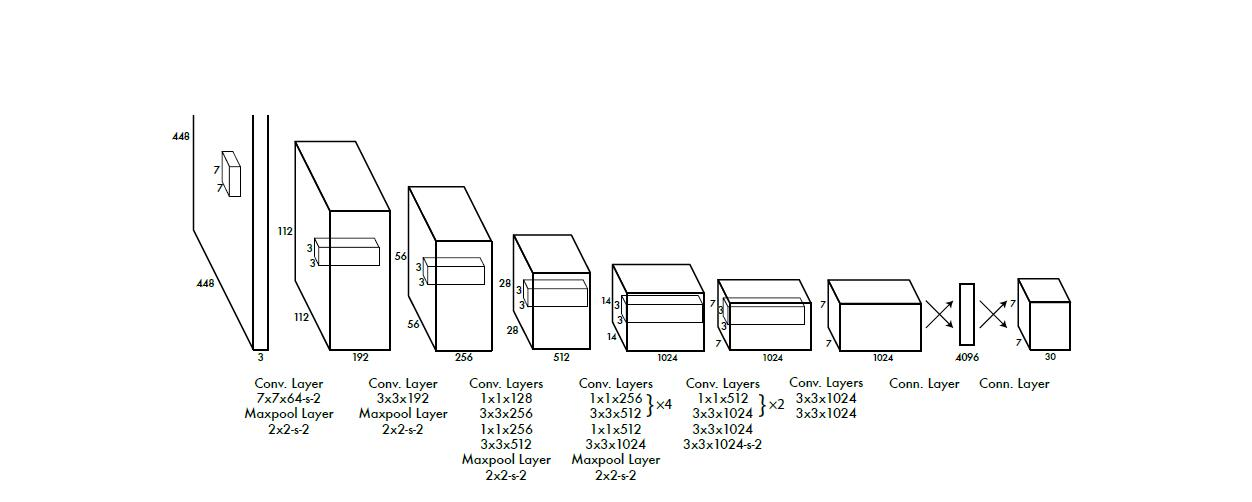
\includegraphics[width=\textwidth]{problem-117_b.jpg}
	\caption{The network architecture for image classification}
\end{figure}
The detection newtork for classification has 24 convolutional layers, then 2 fully connected layers. The output of the overall network is $ 7 \times 7 \times 30$ tensor of predictions.
\subsubsection*{Error and Loss function}
\par YOLO uses sum-squared error as its loss function to optimize the model parameters namely the error of $S \times S \times (B \times 5 + C)=1470$ dimension vector between the network output and real image. 
The loss function is defined as
$$
\operatorname{loss}=\sum_{i=0}^{S^{2}} \text { coord Error }+\text { iou Error }+\text { class Error }
$$
\par Since corrdinate error and intersection-over-union error contributes differently with class error. $\lambda_{\text {coord }}=5$ is added to remedy for corrdinate error.
\par When evaluating intersection-over-union error, cells containing and not containing objects contributes differently to loss function. If they share the same gradient, it pushes the confidence scores of cells that do not contain objects to zero, raising the gradient for cells do contain objects. $\lambda_{\text {noobj }}=0.5$ is added.
The final loss function is ~\cite{redmon2015look}
$$
\begin{aligned} \lambda_{\text {coord }} \sum_{i=0}^{S^{2}} \sum_{j=0}^{B} \mathbb{1}_{i j}^{\text {obj }}\left[\left(x_{i}-\hat{x}_{i}\right)^{2}+\left(y_{i}-\hat{y}_{i}\right)^{2}\right] \\+\lambda_{\text {coord }} \sum_{i=0}^{S^{2}} \sum_{j=0}^{B} \mathbb{1}_{i j}^{\text {obj }}\left[(\sqrt{w_{i}}-\sqrt{\hat{w}_{i}})^{2}+(\sqrt{h_{i}}-\sqrt{\hat{h}_{i}})^{2}\right] \\+\sum_{i=0}^{S^{2}} \sum_{j=0}^{B} \mathbb{1}_{i j}^{\text {obj }}\left(C_{i}-\hat{C}_{i}\right)^{2} \\+\lambda_{\text {noobj }} \sum^{S^{2}}_{i=0} \sum_{j=0}^{B} \mathbb{1}_{i j}^{\text {nobj }}\left(C_{i}-\hat{C}_{i}\right)^{2} \\ +\sum_{i=0}^{S^{2}} \mathbb{I}_{i}^{\text {obj }} \sum_{c \in \text { classes }}\left(p_{i}(c)-\hat{p}_{i}(c)\right)^{2} \end{aligned}
$$
where $\mathbb{1}_{i}^{\mathrm{obj}}$ denotes if object appears in cell $i$, $\mathbb{1}_{ij}^{\mathrm{obj}}$ denotes that the $j$th bounding box predictor in cell $i$ is taken into consideration for that prediction.
\subsubsection*{Training}
\par The training of YOLO model is seperated into two steps. In the pre-training process, the convolutional layers are trained based on the ImageNet 1000-class competition dataset. The first 20 convolutional layers, an average-pooling layer and a fully connected layer is used. Joseph Redmon and his team did the training for around one week, getting an outcome of 88\% accuracy towards the ImageNet 2012 validation set. ~\cite{redmon2015look}
\par In the following step, the resolution of the input image is increased from $224\times 224$ to $448 \times 448$ for fine-grained visual information. The last four convolutional layers and two fully connected layers are added and then initialized with random weights.
\par The linear activation function for all layers is 
$$
\phi(x)=\left\{\begin{array}{ll}{x,} & {\text { if } x>0} \\ {0.1 x,} & {\text { otherwise }}\end{array}\right.
$$
Then, optimize for sum-squared error in the output.

\subsubsection*{Limitations}
YOLO model has its limitations as followed when in practical use. ~\cite{redmon2015look}
\begin{itemize}
	\item YOLO does not perform well in detecting small objects that exist in the image in group, like flock of birds. 
	\item YOLO does poorly in generalization to objects that is unusual.
	\item YOLO has low accuracy in objects localizations.
\end{itemize}
% add comment in the pseudocode: \cmt{comment}
% define a function name: \SetKwFunction{shortname}{Name of the function}
% use the defined function: \shortname{$variables$}
% use the keyword ``function'': \Fn{function name}, e.g. \Fn{\shortname{$var$}}



% include references where to find information on the given problem using latex bibliography
% insert references in the text (\cite{}) and write bibliography file in problem-nb.bib (replace nb with the problem number)
% prefer books, research articles, or internet sources that are likely to remain available over time
% as much as possible offer several options, including at least one which provide a detailed study of the problem
% if available include links to programs/code solving the problem
% wikipedia is NOT acceptable as a unique reference
\singlespacing
\printbibliography[title={References.},resetnumbers=true,heading=subbibliography]

\end{document}
